% Figure 4: Answer word divergence — Venn diagram with semantic distance annotation
% Hunt 1 vs Hunt 2, Jaccard = 0.00, three domain-adjacent pairs annotated.
\begin{figure}[t]
\centering
\usetikzlibrary{arrows.meta, positioning, shapes.geometric, calc}%
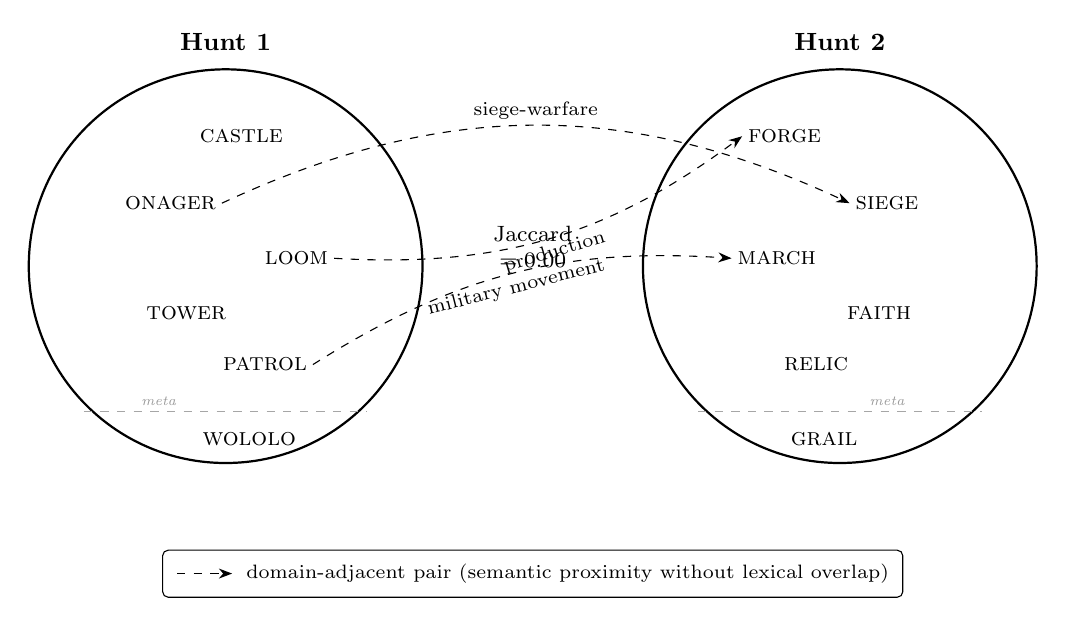
\begin{tikzpicture}[
  >=Stealth,
  font=\small,
  every node/.style={inner sep=2pt},
]

% ── Layout constants ──────────────────────────────────────────────────────────
% Circle radius and horizontal gap between circle edges
\def\R{2.5}         % circle radius (cm)
\def\gap{2.8}       % gap between the two circle edges (cm)
\def\cx{3.9}        % x-coordinate of each circle centre (± from origin)

% ── Hunt 1 circle (left) ─────────────────────────────────────────────────────
\draw[thick] (-\cx, 0) circle (\R);
\node[font=\bfseries\small] at (-\cx, \R+0.35) {Hunt 1};

% Feeder words — Hunt 1
% Positions are hand-placed inside the circle; meta below dashed rule
\node (C1) at (-\cx+0.2,  1.65) {\textsc{castle}};
\node (O1) at (-\cx-0.7,  0.80) {\textsc{onager}};
\node (L1) at (-\cx+0.9,  0.10) {\textsc{loom}};
\node (T1) at (-\cx-0.5, -0.60) {\textsc{tower}};
\node (P1) at (-\cx+0.5, -1.25) {\textsc{patrol}};

% Dashed horizontal rule inside circle (meta separator)
\draw[dashed, gray!70, thin]
  (-\cx-1.8, -1.85) -- (-\cx+1.8, -1.85);
\node[gray!80, font=\tiny\itshape] at (-\cx-0.85, -1.72) {meta};

% Meta answer — Hunt 1
\node (W1) at (-\cx+0.3, -2.20) {\textsc{wololo}};

% ── Hunt 2 circle (right) ────────────────────────────────────────────────────
\draw[thick] (\cx, 0) circle (\R);
\node[font=\bfseries\small] at (\cx, \R+0.35) {Hunt 2};

% Feeder words — Hunt 2
\node (F2) at (\cx-0.7,  1.65) {\textsc{forge}};
\node (S2) at (\cx+0.6,  0.80) {\textsc{siege}};
\node (M2) at (\cx-0.8,  0.10) {\textsc{march}};
\node (A2) at (\cx+0.5, -0.60) {\textsc{faith}};
\node (R2) at (\cx-0.3, -1.25) {\textsc{relic}};

% Dashed horizontal rule inside circle (meta separator)
\draw[dashed, gray!70, thin]
  (\cx-1.8, -1.85) -- (\cx+1.8, -1.85);
\node[gray!80, font=\tiny\itshape] at (\cx+0.60, -1.72) {meta};

% Meta answer — Hunt 2
\node (G2) at (\cx-0.2, -2.20) {\textsc{grail}};

% ── Gap label ────────────────────────────────────────────────────────────────
\node[align=center, font=\footnotesize] at (0, 0.25)
  {Jaccard\\$= 0.00$};

% ── Domain-adjacent arrows ───────────────────────────────────────────────────
% All three are thin, dashed, curved, with midpoint label.
% Arrow: ONAGER (Hunt1) → SIEGE (Hunt2)   "siege-warfare"
\draw[->, dashed, thin, bend left=25]
  (O1.east) to
  node[above, font=\scriptsize, midway, sloped] {siege-warfare}
  (S2.west);

% Arrow: LOOM (Hunt1) → FORGE (Hunt2)   "production"
\draw[->, dashed, thin, bend right=20]
  (L1.east) to
  node[below, font=\scriptsize, midway, sloped] {production}
  (F2.west);

% Arrow: PATROL (Hunt1) → MARCH (Hunt2)   "military movement"
\draw[->, dashed, thin, bend left=18]
  (P1.east) to
  node[below, font=\scriptsize, midway, sloped] {military movement}
  (M2.west);

% ── Legend ───────────────────────────────────────────────────────────────────
\node[
  draw, rounded corners=2pt, inner sep=5pt,
  font=\scriptsize, align=left,
  below=0.55cm of {(-\cx/2, -\R-0.1)},   % centred below the figure
  anchor=north,
] at (0, -\R-0.55)
  {\hspace{0pt}%
   \tikz{\draw[->, dashed, thin] (0,0) -- (0.7,0);}\;
   domain-adjacent pair (semantic proximity without lexical overlap)};

\end{tikzpicture}

\caption{Answer word sets for Hunt~1 (left) and Hunt~2 (right). Exact string
Jaccard $= 0.00$ --- zero shared words across all six slots including the meta
answers. Despite complete lexical divergence, three of five feeder slots
produced domain-adjacent pairs (dashed arrows), suggesting that the AoE2
domain acts as a semantic basin of attraction even when it cannot force exact
word convergence.}
\label{fig:answers}
\end{figure}
